\chapter{Carbonilas conjugadas: Michael e Robinson}\label{ch:b2:conjugate-additions}

Os quatro anéis de um hormônio esteroide foram montados de início um anel de cada vez, e uma
sequência de reações tornou-se a maneira padrão de acrescentar um anel: ela constrói um anel inteiro
de seis membros, cetona incluída, a partir de uma cetona e de uma pequena cetona insaturada. Ela
funciona porque um grupo carbonila conjugado com uma ligação dupla \ce{C=C} transmite seu caráter
eletrofílico à extremidade distante dessa ligação dupla. Este capítulo trata dessa extremidade
distante: que nucleófilos a atacam, por quê, e o que se pode construir com ela.

\begin{recall}
\Cref{ch:b2:enolates-aldol}: \omterm{def:b2:enolates-aldol:enolate}{enolatos}, a \omterm{def:b2:enolates-aldol:aldol}{condensação aldólica}. \Cref{ch:b2:frontier-orbitals}: \omterm{def:b2:frontier-orbitals:control}{controle
de carga} e \omterm{def:b2:frontier-orbitals:control}{controle orbital}, reagentes duros e moles. \Cref{ch:b2:huckel}: orbitais de Hückel e cargas
$\pi$. O volume do 1.º ano: reagentes de Grignard e hidretos, controle cinético e termodinâmico,
sistemas conjugados.
\end{recall}

\section{Dois sítios eletrofílicos}

\begin{definition}[Compostos carbonílicos $\alpha,\beta$-insaturados]\label{def:b2:conjugate-additions:enone}
Um \emph{composto carbonílico $\alpha,\beta$-insaturado}\index{composto carbonilico alfa,beta-insaturado@composto carbonílico $\alpha,\beta$-insaturado}
tem uma ligação dupla \ce{C=C} entre os carbonos $\alpha$
e $\beta$ de um composto carbonílico, conjugada com a \ce{C=O}: uma enona (cetona), um enal
(aldeído), um éster ou uma \omterm{def:b2:amines:nitrile}{nitrila} insaturados. Os mais simples são o propenal \ce{CH2=CHCHO} e a
but-3-en-2-ona \ce{CH2=CHCOCH3} (metilvinilcetona).
\end{definition}

\begin{omfigure}
\setchemfig{atom sep=1.9em}
\schemestart
\chemfig{H_2C=CH-CH=O}
\arrow{<->}
\chemfig{H_2C=CH-\chemabove{C}{\scriptstyle +}H-\chemabove{O}{\scriptstyle -}}
\arrow{<->}
\chemfig{\chemabove{C}{\scriptstyle +}H_2-CH=CH-\chemabove{O}{\scriptstyle -}}
\schemestop
\par\medskip

\begin{tikzpicture}
\begin{axis}[ybar, width=0.47\linewidth, height=4.6cm, ymin=-0.6, ymax=0.4,
  xtick={1,2,3,4}, xticklabels={C$\beta$,C$\alpha$,C(O),O}, axis x line=bottom, axis y line=left,
  extra y ticks={0}, extra y tick style={grid=major, grid style={black!50}}, enlarge x limits=0.15,
  tick label style={font=\scriptsize}, ylabel={carga $\pi$}, label style={font=\small},
  title={\small Cargas $\pi$ do propenal}, bar width=8pt]
\addplot[fill=omDef!50, draw=omDef] table[x=atom, y=q] {figdata/out/bachelor-2-huckel-d.dat};
\end{axis}
\end{tikzpicture}\hfill
\begin{tikzpicture}
\begin{axis}[ybar, width=0.47\linewidth, height=4.6cm, ymin=-0.8, ymax=0.8,
  xtick={1,2,3,4}, xticklabels={C$\beta$,C$\alpha$,C(O),O}, axis x line=bottom, axis y line=left,
  extra y ticks={0}, extra y tick style={grid=major, grid style={black!50}}, enlarge x limits=0.15,
  tick label style={font=\scriptsize}, ylabel={coeficiente}, label style={font=\small},
  title={\small LUMO do propenal}, bar width=8pt]
\addplot[fill=omThm!45, draw=omThm] table[x=atom, y=c] {figdata/out/bachelor-2-huckel-d.dat};
\end{axis}
\end{tikzpicture}

{\small O propenal. Em cima: suas três estruturas de ressonância; as duas últimas põem uma carga
positiva no carbono carbonílico e no carbono $\beta$. Embaixo: o modelo de Hückel do
\cref{ch:b2:frontier-orbitals} ($\alpha_{\ce{O}} = \alpha + \beta$, $\beta_{\ce{CO}} = \beta$; um modelo).
A maior carga positiva está no carbono carbonílico (+0.33, contra +0.23 no carbono $\beta$); o maior
coeficiente da \omterm{def:b2:frontier-orbitals:frontier}{LUMO} está no carbono $\beta$ (0.66, contra $-0.58$).}
\end{omfigure}

\begin{proposition}[Dois sítios]\label{prop:b2:conjugate-additions:two-sites}
Em um composto carbonílico $\alpha,\beta$-insaturado, tanto o carbono carbonílico quanto o carbono
$\beta$ são eletrofílicos. O carbono carbonílico leva a maior carga positiva; o carbono $\beta$ leva o
maior coeficiente na \omterm{def:b2:frontier-orbitals:frontier}{LUMO}.
\end{proposition}

\begin{proof}[Raciocínio]
As estruturas de ressonância colocam uma carga positiva no carbono carbonílico e, através da \ce{C=C},
no carbono $\beta$; o carbono $\alpha$ nunca é positivo. O modelo de Hückel do propenal torna isso
quantitativo: somando $2c^2$ sobre os dois orbitais $\pi$ ocupados obtêm-se as cargas $\pi$
(\cref{def:b2:huckel:indices}) $+0.33$ no carbono carbonílico, $+0.23$ no carbono $\beta$, $-0.03$
no carbono $\alpha$ e $-0.53$ no oxigênio. A \omterm{def:b2:frontier-orbitals:frontier}{LUMO}, o orbital que recebe os elétrons de um nucleófilo,
é máxima no carbono $\beta$. Os dois sítios respondem portanto aos dois tipos de controle
da \cref{def:b2:frontier-orbitals:control}.
% figdata: bachelor-2/huckel.py part d
\end{proof}

\section{Adição 1,2 ou adição conjugada}

\begin{definition}[Modos de adição]\label{def:b2:conjugate-additions:addition-modes}
Um nucleófilo que se adiciona ao carbono carbonílico de um composto carbonílico $\alpha,\beta$-insaturado
dá uma \emph{adição 1,2}\index{adicao 1,2@adição 1,2} (contando a partir do oxigênio): um alcóxido alílico, depois um
álcool. Um nucleófilo que se adiciona ao carbono $\beta$ dá uma \emph{adição conjugada}\index{adicao conjugada@adição conjugada}
(ou adição 1,4): um \omterm{def:b2:enolates-aldol:enolate}{enolato}, que é protonado no carbono, dando um composto carbonílico saturado
substituído no carbono $\beta$.
\end{definition}

\begin{omfigure}
\setchemfig{atom sep=1.9em}
\schemestart
\chemfig{*6(-=-(=O)---)}
\arrow{->[\ce{CH3Li}][depois \ce{H2O}]}[,1.4]
\chemfig{*6(-=-(-[:75]CH_3)(-[:-15]OH)---)}
\schemestop
\hspace{2.5em}
\schemestart
\chemfig{*6(-=-(=O)---)}
\arrow{->[\ce{(CH3)2CuLi}][depois \ce{H2O}]}[,1.6]
\chemfig{*6(-(-CH_3)--(=O)---)}
\schemestop
\par\vspace{6pt}

{\small A ciclo-hex-2-en-1-ona com dois nucleófilos metila. O metil-lítio, um \omterm{def:b2:frontier-orbitals:hard-soft}{nucleófilo duro}, se
adiciona ao carbono carbonílico: 1-metilciclo-hex-2-en-1-ol (\omterm{def:b2:conjugate-additions:addition-modes}{adição 1,2}). O dimetilcuprato de lítio,
um \omterm{def:b2:frontier-orbitals:hard-soft}{nucleófilo mole}, se adiciona ao carbono $\beta$: 3-metilciclo-hexanona (\omterm{def:b2:conjugate-additions:addition-modes}{adição conjugada}).}
\end{omfigure}

\begin{proposition}[Que sítio]\label{prop:b2:conjugate-additions:regio}
Os \omterm{def:b2:frontier-orbitals:hard-soft}{nucleófilos duros} (organolítios, a maioria dos reagentes de Grignard, \ce{LiAlH4}) se adicionam
sobretudo em 1,2, sob \omterm{def:b2:frontier-orbitals:control}{controle de carga}, em geral de modo irreversível. Os \omterm{def:b2:frontier-orbitals:hard-soft}{nucleófilos moles}
(\omterm{def:b2:conjugate-additions:cuprate}{organocupratos}, \omterm{def:b2:enolates-aldol:enolate}{enolatos} estabilizados, tiolatos, aminas) se adicionam sobretudo em 1,4, sob
\omterm{def:b2:frontier-orbitals:control}{controle orbital}; o aduto conjugado, que conserva a ligação \ce{C=O}, é também o produto mais estável.
\end{proposition}

\begin{proof}[Raciocínio]
Um \omterm{def:b2:frontier-orbitals:hard-soft}{nucleófilo duro}, pequeno e carregado, interage sobretudo por meio das cargas: ele vai ao centro
mais positivo, o carbono carbonílico (\cref{prop:b2:conjugate-additions:two-sites}); sua adição é
rápida e não se reverte, de modo que o produto 1,2, formado mais depressa, permanece (controle
cinético). Um \omterm{def:b2:frontier-orbitals:hard-soft}{nucleófilo mole}, grande e polarizável, com uma \omterm{def:b2:frontier-orbitals:frontier}{HOMO} alta, interage sobretudo por meio
dos \omterm{def:b2:frontier-orbitals:frontier}{orbitais de fronteira}: ele vai aonde a \omterm{def:b2:frontier-orbitals:frontier}{LUMO} é máxima, o carbono $\beta$. O produto 1,4 conserva
uma ligação $\pi$ \ce{C=O}, mais forte que a ligação $\pi$ \ce{C=C} conservada pelo produto 1,2;
quando as adições são reversíveis (cianeto, aminas, \omterm{def:b2:enolates-aldol:enolate}{enolatos} estabilizados, alcóxidos), o equilíbrio
deriva portanto para o aduto conjugado, mesmo quando o aduto 1,2 se formou primeiro (controle
termodinâmico).
\end{proof}

\begin{method}[Prever o modo de adição]\label{met:b2:conjugate-additions:predict-mode}
\begin{enumerate}
  \item Classifique o nucleófilo: duro (\ce{RLi}, \ce{RMgX}, \ce{LiAlH4}, \ce{NaBH4} com um aldeído)
        ou mole (\ce{R2CuLi}, um \omterm{def:b2:enolates-aldol:enolate}{enolato} 1,3-dicarbonílico, \ce{RS-}, \ce{R2NH}, cianeto no equilíbrio).
  \item Verifique a reversibilidade: uma adição dura irreversível dá o produto 1,2; uma reversível dá,
        com o tempo, o produto 1,4.
  \item Verifique o impedimento: um carbono $\beta$ substituído retarda a adição 1,4; um aldeído, menos
        impedido e mais reativo em sua carbonila que uma cetona, favorece 1,2.
  \item Escreva o \omterm{def:b2:enolates-aldol:enolate}{enolato} formado pela adição 1,4: ele pode ser protonado, ou capturado por um
        eletrófilo.
\end{enumerate}
\end{method}

\section{As adições de Michael}

\begin{definition}[Adição de Michael]\label{def:b2:conjugate-additions:michael}
Uma \emph{adição de Michael}\index{adicao de Michael@adição de Michael} é a \omterm{def:b2:conjugate-additions:addition-modes}{adição conjugada} de um carbânion estabilizado,
em geral um \omterm{def:b2:enolates-aldol:enolate}{enolato}, a um composto carbonílico $\alpha,\beta$-insaturado ou a um alceno pobre em
elétrons semelhante. O nucleófilo é o \emph{doador de Michael}\index{doador de Michael} (um composto 1,3-dicarbonílico, um
nitroalcano, um cianoéster); o composto insaturado é o \emph{aceptor de Michael}\index{aceptor de Michael}
(uma enona, um enal, um éster, uma \omterm{def:b2:amines:nitrile}{nitrila} ou um composto nitro insaturados).
\end{definition}

\begin{omfigure}
\setchemfig{atom sep=1.8em}
\schemestart
\chemfig{CH_2(-[:30]COOEt)(-[:-30]COOEt)}
\arrow{<=>[\ce{EtO-}][$-$ \ce{EtOH}]}[,1.3]
\chemfig{\chemabove{C}{\scriptstyle -}H(-[:30]COOEt)(-[:-30]COOEt)}
\+
\chemfig{H_2C=CH-C(=[2]O)-CH_3}
\schemestop

\medskip
\setchemfig{atom sep=1.6em}
\schemestart
\arrow{->[adição]}[,0.95]
\chemfig{CH(-[:150]EtOOC)(-[:210]EtOOC)-CH_2-CH=C(-[2]\chemabove{O}{\scriptstyle -})-CH_3}
\arrow{->[\ce{EtOH}][$-$ \ce{EtO-}]}[,1.1]
\chemfig{CH(-[:150]EtOOC)(-[:210]EtOOC)-CH_2-CH_2-C(=[2]O)-CH_3}
\schemestop
\par\vspace{6pt}

{\small A \omterm{def:b2:conjugate-additions:michael}{adição de Michael} do propanodioato de dietila à but-3-en-2-ona. O etóxido forma o \omterm{def:b2:enolates-aldol:enolate}{enolato}
estabilizado; este se adiciona ao carbono $\beta$; o \omterm{def:b2:enolates-aldol:enolate}{enolato} formado toma um próton do etanol, o que
regenera o etóxido. O produto, o (3-oxobutil)propanodioato de dietila, é um composto
1,5-dicarbonílico.}
\end{omfigure}

\begin{proposition}[Mecanismo de Michael]\label{prop:b2:conjugate-additions:michael}
Uma \omterm{def:b2:conjugate-additions:michael}{adição de Michael} ocorre em três etapas (desprotonação do doador, \omterm{def:b2:conjugate-additions:addition-modes}{adição conjugada}, protonação do
novo \omterm{def:b2:enolates-aldol:enolate}{enolato}), e a base é regenerada na última etapa: uma quantidade catalítica basta.
\end{proposition}

\begin{proof}[Raciocínio]
O hidrogênio $\alpha$ do doador, entre duas carbonilas, é ácido: $\mathrm pK_a$ cerca de 13 para o
propanodioato de dietila, 10.7 para o 3-oxobutanoato de etila. O etóxido (etanol, 15.9) o retira em
grande parte, o que é mais que suficiente. O \omterm{def:b2:enolates-aldol:enolate}{enolato} estabilizado, mole, se adiciona em 1,4
(\cref{prop:b2:conjugate-additions:regio}). O \omterm{def:b2:enolates-aldol:enolate}{enolato} formado é uma base mais forte que o \omterm{def:b2:enolates-aldol:enolate}{enolato} do
doador (ele é estabilizado por uma carbonila, não duas), de modo que toma um próton do solvente,
devolvendo um etóxido para o que foi consumido. A reação global forma uma ligação $\sigma$ \ce{C-C} a
partir de uma ligação $\pi$ \ce{C=C}: ela é favorável, e com um doador estabilizado o aduto não se reverte.
% ledger: pka:ethanol, pka:diethylmalonate, pka:acetoacetate
\end{proof}

Um aduto de Michael com uma cetona do lado do doador e outra do lado do aceptor é um composto
1,5-dicarbonílico: as duas carbonilas estão a cinco carbonos uma da outra, contando os dois carbonos
carbonílicos. Esse padrão é a assinatura de uma \omterm{def:b2:conjugate-additions:michael}{adição de Michael}, como a carbonila $\beta$-hidroxilada
era a da \omterm{def:b2:enolates-aldol:aldol}{aldólica} (\cref{met:b2:enolates-aldol:aldol-recognition}).

\section{Os organocupratos}

\begin{definition}[Organocupratos]\label{def:b2:conjugate-additions:cuprate}
Um \emph{organocuprato}\index{organocuprato} \ce{R2CuLi} é um composto de cobre(I) que leva dois grupos
orgânicos, preparado a partir de dois equivalentes de um organolítio e um de um haleto de cobre(I):
\begin{equation*}
\ce{2 CH3Li + CuI -> (CH3)2CuLi + LiI}.
\end{equation*}
\end{definition}

Os \omterm{def:b2:conjugate-additions:cuprate}{organocupratos} (também chamados reagentes de Gilman) são preparados e usados em éter a baixa
temperatura sob gás inerte, como seus parentes organolítios. O cobre é menos eletropositivo que o lítio
ou o magnésio, de modo que a ligação \ce{Cu-C} é mais covalente e o carbono menos carregado: o grupo
metila de um cuprato é um \omterm{def:b2:frontier-orbitals:hard-soft}{nucleófilo mole}. Daí três usos.

\begin{itemize}
  \item \emph{\omterm{def:b2:conjugate-additions:addition-modes}{Adição conjugada}} de um grupo alquila ou arila a uma enona, o que os reagentes de Grignard e
        os organolítios não fazem de modo limpo; só um dos dois grupos \ce{R} é transferido.
  \item \emph{Captura}: o \omterm{def:b2:enolates-aldol:enolate}{enolato} formado pela \omterm{def:b2:conjugate-additions:addition-modes}{adição conjugada} pode ser alquilado em seu carbono
        $\alpha$, de modo que duas novas ligações \ce{C-C} são criadas em uma só operação.
  \item \emph{Substituição} de haletos: $\mathrm{R_2CuLi + R'Br \to R{-}R' + RCu + LiBr}$, um acoplamento que um
        organolítio estragaria por eliminação ou troca.
\end{itemize}

\section{A anelação de Robinson}

\begin{definition}[Anelação]\label{def:b2:conjugate-additions:robinson}
Uma \emph{anelação}\index{anelacao@anelação} constrói um novo anel sobre uma molécula existente. A \emph{anelação de Robinson}
\index{anelacao de Robinson@anelação de Robinson} constrói uma ciclo-hex-2-en-1-ona: uma \omterm{def:b2:conjugate-additions:michael}{adição de Michael} do
\omterm{def:b2:enolates-aldol:enolate}{enolato} de uma cetona a uma cetona $\alpha,\beta$-insaturada (tipicamente a but-3-en-2-ona), seguida de
uma \omterm{def:b2:enolates-aldol:aldol}{condensação aldólica} intramolecular da 1,5-dicetona formada.
\end{definition}

\begin{omfigure}
\setchemfig{atom sep=1.8em}
\schemestart
\chemfig{[:30]*6(-(=O)-(-CH_3)-(=O)---)}
\+
\chemfig{=[:30]-[:-30](=[:-90]O)-[:30]}
\arrow{->[base][Michael]}[,1.2]
\chemfig{[:30]*6(-(=O)-(-[:40]CH_3)(-[:-30]-[:30]-[:-30](=[:-90]O)-[:30])-(=O)---)}
\schemestop

\medskip
\schemestart
\arrow{->[base][aldólica]}[,1.1]
\chemfig{[:-30]*6(---(-[:-60]OH)*6(--(=O)---)-(-[:105]CH_3)-(=O)-)}
\arrow{->[calor][$-$ \ce{H2O}]}[,1.1]
\chemfig{[:-30]*6(---*6(=-(=O)---)-(-[:105]CH_3)-(=O)-)}
\schemestop
\par\vspace{6pt}

{\small A \omterm{def:b2:conjugate-additions:robinson}{anelação de Robinson} que fornece a cetona de Wieland--Miescher. O \omterm{def:b2:enolates-aldol:enolate}{enolato} da
2-metilciclo-hexano-1,3-diona se adiciona à but-3-en-2-ona (Michael): uma tricetona. O \omterm{def:b2:enolates-aldol:enolate}{enolato} da
metilcetona da cadeia lateral ataca uma carbonila do anel (\omterm{def:b2:enolates-aldol:aldol}{aldólica} intramolecular), fechando um anel
de seis membros; a desidratação dá a enona conjugada. O grupo metila angular fica no carbono comum
aos dois anéis, o único estereocentro.}
\end{omfigure}

\begin{proposition}[Anelação de Robinson]\label{prop:b2:conjugate-additions:robinson}
Uma cetona com um hidrogênio $\alpha$ e a but-3-en-2-ona, em meio básico, dão uma ciclo-hex-2-en-1-ona
em três etapas: \omterm{def:b2:conjugate-additions:michael}{adição de Michael}, \omterm{def:b2:enolates-aldol:aldol}{adição aldólica} intramolecular formando um anel de seis membros, e
desidratação. O novo anel contém o antigo carbono $\alpha$ da cetona e seu carbono carbonílico, e os
quatro carbonos da but-3-en-2-ona.
\end{proposition}

\begin{proof}
Siga os átomos na figura. O carbono do \omterm{def:b2:enolates-aldol:enolate}{enolato} da cetona (chamemo-lo C$_a$) se liga ao carbono $\beta$
da but-3-en-2-ona: a cadeia C$_a$--\ce{CH2}--\ce{CH2}--\ce{C(=O)}--\ce{CH3} fica pendurada em C$_a$, e
C$_a$ continua ligado ao carbono carbonílico C$_k$ da cetona. Em meio básico, a metilcetona da cadeia
forma seu \omterm{def:b2:enolates-aldol:enolate}{enolato} no \ce{CH3} terminal, que ataca C$_k$. O anel fechado conta C$_k$, C$_a$,
os dois \ce{CH2}, o carbono carbonílico da cadeia lateral e o antigo carbono metílico: seis átomos, o
tamanho de anel sem tensão, e é por isso que esse \omterm{def:b2:enolates-aldol:enolate}{enolato}, entre os possíveis, leva a um produto estável
(um ataque pelo \omterm{def:b2:enolates-aldol:enolate}{enolato} do \ce{CH2} interno da cadeia fecharia um anel de quatro membros). O \omterm{def:b2:enolates-aldol:aldol}{aldol} tem
seu \ce{OH} em C$_k$, em $\beta$ da carbonila da cadeia; a desidratação coloca a \ce{C=C} entre C$_k$ e
o antigo carbono metílico, conjugada com a carbonila: uma ciclo-hex-2-en-1-ona.
\end{proof}

\begin{method}[Desconectar uma ciclo-hexenona]\label{met:b2:conjugate-additions:robinson-disconnection}
\begin{enumerate}
  \item Encontre uma ciclo-hex-2-en-1-ona no alvo; numere seu carbono carbonílico C1, a ligação dupla
        C2=C3, e o anel até C6.
  \item Desfaça a desidratação: um \ce{OH} em C3, uma \ce{C-H} em C2.
  \item Desfaça a \omterm{def:b2:enolates-aldol:aldol}{aldólica}: corte C2--C3. C3 torna-se uma carbonila de cetona, C2 o grupo metila de
        uma metilcetona: uma 1,5-dicetona.
  \item Desfaça a \omterm{def:b2:conjugate-additions:michael}{adição de Michael}: corte a ligação entre C4 (o carbono $\alpha$ da cetona em C3) e
        C5. O doador é essa cetona; o aceptor é a enona C5=C6--C1(=O)--C2, que é a
        but-3-en-2-ona quando C5, C6 e C2 só levam hidrogênios.
\end{enumerate}
\end{method}

\begin{history}[A anelação, 1935]
\begin{minipage}[t]{0.18\linewidth}
\vspace{0pt}
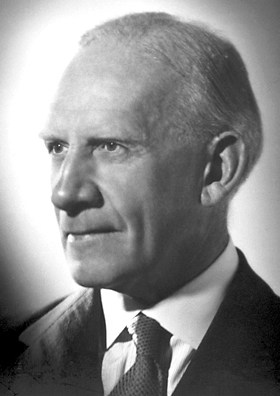
\includegraphics[width=\linewidth]{images/book3/robinson.jpg}
\end{minipage}\hfill
\begin{minipage}[t]{0.78\linewidth}
\vspace{0pt}
Robert Robinson e William Rapson publicaram a sequência de formação de anel em 1935, em trabalhos
voltados para a síntese dos esteroides. As principais realizações de Robinson foram as estruturas e
sínteses de alcaloides, pelas quais ele recebeu o Prêmio Nobel de Química de 1947. Em 1950, Peter
Wieland e Karl Miescher prepararam a dicetona bicíclica do problema deste capítulo, que se tornou um
ponto de partida comum para sínteses de esteroides e terpenos. (Retrato: autor desconhecido, domínio
público; Wikimedia Commons.)
\end{minipage}
\end{history}

\begin{safety}{\ghs[5mm]{GHS02}\,\ghs[5mm]{GHS05}\,\ghs[5mm]{GHS06}\,\ghs[5mm]{GHS07}\,\ghs[5mm]{GHS08}\,\ghs[5mm]{GHS09}}
A but-3-en-2-ona é inflamável, muito tóxica, corrosiva e perigosa para o meio aquático, além de ser um
lacrimogêneo poderoso; ela só é manuseada na capela. A ciclo-hex-2-en-1-ona é inflamável e tóxica. Os
organolítios, os reagentes de Grignard e os cupratos reagem violentamente com a água e são manuseados
sob gás inerte.
% ledger: ghs:MVK, ghs:cyclohexenone, ghs:MeMgBr
\end{safety}

\section{Exercícios}

\begin{exercise}[$\star$]\label{exo:b2:conjugate-additions:1}
Preveja \omterm{def:b2:conjugate-additions:addition-modes}{adição 1,2} ou 1,4 à ciclo-hex-2-en-1-ona para: \ce{CH3MgBr}; \ce{(CH3)2CuLi};
\ce{C6H5SH} com um pouco de base; \ce{LiAlH4}.
\end{exercise}

\begin{exercise}[$\star$]\label{exo:b2:conjugate-additions:2}
Classifique como doador ou \omterm{def:b2:conjugate-additions:michael}{aceptor de Michael}: pentano-2,4-diona, propenonitrila \ce{CH2=CHCN},
nitrometano, propenoato de metila, propanodioato de dietila, but-3-en-2-ona.
\end{exercise}

\begin{exercise}[$\star$]\label{exo:b2:conjugate-additions:3}
Escreva a preparação do dibutilcuprato de lítio a partir do 1-bromobutano, do lítio e do iodeto de cobre(I).
\end{exercise}

\begin{exercise}[$\star$]\label{exo:b2:conjugate-additions:4}
Dê o produto do propanodioato de dietila com a but-3-en-2-ona e uma quantidade catalítica de etóxido
de sódio, e depois o produto após hidrólise e aquecimento.
\end{exercise}

\begin{exercise}[$\star\star$]\label{exo:b2:conjugate-additions:5}
Proponha uma preparação da 3-metilciclo-hexanona a partir da ciclo-hex-2-en-1-ona, e explique por que
o brometo de metilmagnésio seria uma má escolha.
\end{exercise}

\begin{exercise}[$\star\star$]\label{exo:b2:conjugate-additions:6}
O etanotiol se adiciona à but-3-en-2-ona com um traço de trietilamina. Escreva o mecanismo e diga por
que o tiolato se adiciona em 1,4.
\end{exercise}

\begin{exercise}[$\star\star$]\label{exo:b2:conjugate-additions:7}
O cianeto com a ciclo-hex-2-en-1-ona dá, a baixa temperatura e em tempos curtos, a cianoidrina; a
temperatura mais alta e em tempos mais longos, a 3-oxociclo-hexano-1-carbonitrila. Explique pelo
controle cinético e termodinâmico.
\end{exercise}

\begin{exercise}[$\star\star$]\label{exo:b2:conjugate-additions:8}
Dê o produto da \omterm{def:b2:conjugate-additions:robinson}{anelação de Robinson} da 2-metilciclo-hexano-1,3-diona com a but-3-en-2-ona, depois o da
ciclo-hexanona com a but-3-en-2-ona.
\end{exercise}

\begin{exercise}[$\star\star$]\label{exo:b2:conjugate-additions:9}
Desconecte a heptano-2,6-diona em um doador e um \omterm{def:b2:conjugate-additions:michael}{aceptor de Michael}, e proponha condições.
\end{exercise}

\begin{exercise}[$\star\star\star$]\label{exo:b2:conjugate-additions:10}
Uma \omterm{def:b2:enolates-aldol:aldol}{adição aldólica} simples se reverte facilmente em meio básico; o aduto de Michael do propanodioato de
dietila e da but-3-en-2-ona, não. Explique pelas ligações formadas e rompidas e pela acidez do produto.
\end{exercise}

\begin{exercise}[$\star\star\star$]\label{exo:b2:conjugate-additions:11}
O propanodioato de dietila com dois equivalentes de propenoato de metila e uma base catalítica dá um
produto sem nenhuma \ce{C-H} restante entre seus dois grupos éster. Desenhe-o e explique.
\end{exercise}

\begin{exercise}[$\star\star\star$]\label{exo:b2:conjugate-additions:12}
A 2-metilciclo-hexanona e a but-3-en-2-ona, em uma \omterm{def:b2:conjugate-additions:robinson}{anelação de Robinson}, podem reagir por qualquer
um dos dois \omterm{def:b2:enolates-aldol:enolate}{enolatos}. Desenhe os dois produtos e diga que condições favorecem aquele que tem o grupo
metila no carbono de fusão dos anéis.
\end{exercise}

\section{Problema: A cetona de Wieland--Miescher}

\begin{problem}[{Problema de fim de semana --- o doador ácido, o aduto de Michael, a aldólica
intramolecular e sua desidratação, o estereocentro e o balanço de massa de uma preparação}]
\label{pb:b2:conjugate-additions:1}
Preparação (dados do exercício): \qty{10.0}{g} de 2-metilciclo-hexano-1,3-diona reagem com um leve
excesso de but-3-en-2-ona e uma base catalítica (\omterm{def:b2:conjugate-additions:michael}{adição de Michael}); a tricetona é depois ciclizada com
uma \omterm{def:b2:amines:class}{amina secundária} e um ácido (\omterm{def:b2:enolates-aldol:aldol}{aldólica}, desidratação). Rendimento global: 70~\%. A
ciclo-hexano-1,3-diona de referência tem $\mathrm pK_a = 5.3$ em água. Massas molares (\unit{g/mol}): C 12.011, H 1.008, O 15.999.
% ledger: pka:cyclohexanedione, aw:C, aw:H, aw:O, ghs:methylcyclohexanedione, ghs:MVK

\medskip
\noindent\textbf{Parte I --- O doador.}
\begin{enumerate}
  \item Desenhe a 2-metilciclo-hexano-1,3-diona e marque seu hidrogênio mais ácido.
  \item Por que esse hidrogênio é tão mais ácido que os hidrogênios $\alpha$ da ciclo-hexanona?
  \item Desenhe as três estruturas de ressonância de seu \omterm{def:b2:enolates-aldol:enolate}{enolato}.
  \item O hidróxido ou o etóxido são fortes o bastante para formar completamente esse \omterm{def:b2:enolates-aldol:enolate}{enolato}? Use o $\mathrm pK_a$.
  \item Escreva o \omterm{def:b2:enolates-aldol:tautomerism}{enol} da diona que envolve C2, e diga por que o grupo metila em C2 não
        o impede.
  \item Esse \omterm{def:b2:enolates-aldol:enolate}{enolato} é duro ou mole? Que sítio da but-3-en-2-ona ele vai atacar?
\end{enumerate}

\medskip
\noindent\textbf{Parte II --- O aduto de Michael.}
\begin{enumerate}[resume]
  \item Escreva a \omterm{def:b2:conjugate-additions:michael}{adição de Michael} e dê o nome da tricetona formada.
  \item Por que basta uma quantidade catalítica de base?
  \item Por que a nova ligação se forma em C2 da diona e não em seu oxigênio?
  \item Quantos carbonos quaternários a tricetona tem?
  \item Identifique a relação 1,5-dicarbonílica na tricetona.
  \item Por que se usa um leve excesso de but-3-en-2-ona, e por que apenas leve?
\end{enumerate}

\medskip
\noindent\textbf{Parte III --- O fechamento do anel.}
\begin{enumerate}[resume]
  \item Liste os carbonos da tricetona que levam hidrogênios $\alpha$.
  \item Que \omterm{def:b2:enolates-aldol:enolate}{enolato}, atacando que carbonila, fecha um anel de seis membros?
  \item Que outros fechamentos de anel poderiam ser tentados, e por que eles não dão o produto?
  \item Escreva o \omterm{def:b2:enolates-aldol:aldol}{aldol} formado e a desidratação que se segue.
  \item Por que a desidratação é fácil?
  \item Dê os grupos funcionais da cetona de Wieland--Miescher.
\end{enumerate}

\medskip
\noindent\textbf{Parte IV --- Estereoquímica e balanço de massa.}
\begin{enumerate}[resume]
  \item Que carbono do produto é um estereocentro?
  \item O produto desta preparação é opticamente ativo? Explique.
  \item Calcule as massas molares da diona, da but-3-en-2-ona e do produto
        \ce{C11H14O2}.
  \item Escreva a equação global e verifique-a com as fórmulas.
  \item Calcule a quantidade de diona usada.
  \item Dê a massa de cetona de Wieland--Miescher obtida com 70~\% de rendimento global.
\end{enumerate}
\end{problem}
